
\chapter{一致性、完全性与几何学}

\section{隐含意义与显明意义}

在第二章里我们看到,当规则支配的符号与真实世界中的事物之间有个同构时,意义——至少在形式系统这种相对简单的语境里——是如何出现的。一般说来,这个同构越复杂,为从符号中抽出意义所需的“设备”——硬的和软的——就越多。若一个同构很简单(或很熟悉),我们倾向于说它相对于我们的意义是显明的。我们不必注意这个同构就见到了意义。最明显的例子是人类的语言,人们常常把意义归于词本身,丝毫没有意识到使词具有意义的那个非常复杂的同构。这是个很容易犯的错误:把全部意义归于对象(即词),而非对象与真实世界的联结。这可以与一种朴素信念作个比较:认为任何两个物体的碰撞都必然附带有声音。这是个错误的信念。当两个物体在真空中相撞时,就不会有任何声音。道理是一样的。错误来自把声音完全归于碰撞,而未看到把声音从对象带给耳朵的媒介的作用。

以前,我让“同构”这个词带上引号是表明必须要留有余地。支持着对人类语言进行理解的符号操作过程,比典型的形式系统中的符号操作过程要复杂得多。因此我们要想继续把意义当作以同构为媒介的,我们就得对于同构能是什么采取更为灵活的看法,事实上在我看来,回答“什么是意识?”这一问题的关键之点,是揭示出作为意义基础的“同构”的实质。

\section{《对位藏头诗》的显明意义}

以上都是在准备对《对位藏头诗》的讨论——一种对于意义层次的研究。这篇对话既有显明的意义也有隐含的意义。最显明的意义无非是它所讲述的故事。严格地说,这个“显明的”意义是极度隐含的,因为面对白纸上的那些黑色印记,要理解故事中的事件,需要复杂得难以想象的大脑过程。尽管如此,我们还是把故事中的事件当作对话的显明意义,并假定每位读者都多少是用同样的“同构”从纸上的印记中抽取出这层意义的。

即便如此,我还是想把那个故事的显明意义说得更明白些。首先我想谈谈唱机与唱片。主要的问题是唱片上的纹道有两层意义。第一层意义是音乐意义。那么什么是“音乐”?——是空气中一系列的震颤,还是大脑中相继的情感反应?两者都是。但在有情感反应之前,先得有震颤。震颤是由唱机从纹道里“抽”出来的:一个相对说来直接了当的机制。事实上你都可以用一根针来做到,只需把针沿着纹道划就行。这个阶段之后,耳朵把震颤转换成大脑中听觉神经元的发射。以后便是大脑中的一系列步骤,逐渐地把线性的震颤序列变换成相互作用着的情感反应的复杂模式——太复杂了,我们不能再深究,虽然我很想这样。所以我们还是满足于把空气中的声音当作纹道的“第一层”意义。

纹道的第二层意义是什么?是在唱机中引起的震颤序列。这层意义只能是在第一层意义从纹道上被抽出来之后才有,因为是空气中的震颤引起了唱机中的震颤。所以,第二层意义有赖于相继的两个同构:
\begin{enumerate}
\item 任意的纹道模式与空气震颤之间的同构;
\item 任意的空气震颤与唱机震颤之间的同构。
\end{enumerate}
这两个相继的同构的示意图见\fig{20}。注意是同构$1$使第一层意义出现。第二层意义比第一层意义隐含一些,因为它的媒介是两个相继同构。就是这第二层意义“倒戈”,才使唱机破碎的。有趣的是第一层意义的产生迫使第二层意义也要同时产生——决不会只有第一层意义而没有第二层。所以,是唱片的隐含意义又转了回来,毁掉了唱片。

\begin{figure}
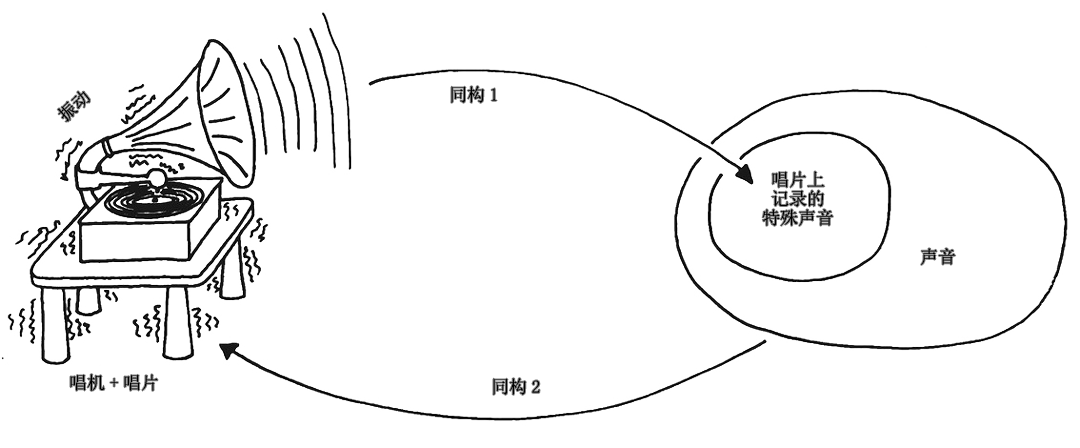
\includegraphics{img_020.png}
\caption[哥德尔定理背后的原理的形象化表现。]
  {哥德尔定理背后的原理的形象化表现:两个映射背靠背具有了出乎意料的飞去来器效果。第一个映射是从纹道模式到声音,由一个唱机实现。第二个——很平常,但却常常被忽视——是从声音到唱机的震颤。注意第二个映射独立于第一个映射而存在,因为附近的任何声音——不仅是唱机自己产生的声音——都会引起这种震颤。哥德尔定理转述在这里就是:对任何一个唱机,都有它不能播放的唱片,因为后者会导致前者的间接自摧毁。[作者绘。]}
\end{figure}

高脚杯的情形是一样的,同样可以这么说。但有个区别:字母表中的字母到音符上的映射是另外一层同构,我们可以称之为“转录”。这个同构之后跟着的是“翻译”——音符到乐音的转换。再之后,震颤反作用到高脚杯上,恰如反作用到那一系列逐步升级的唱机上一样。

\section{《对位藏头诗》的隐含意义}

那篇对话的隐含意义又如何呢?(是的,有不止一层。)其中最简单的已在前面指出了——就是,对话前半部分与后半部分大体上是同构的:唱机变成了小提琴,乌龟变成了阿基里斯,螃蟹变成了乌龟,纹道变成了刻写的签名,等等。注意到了这个简单的同构,你还可以更进一步。注意在故事的前半部分乌龟是全部恶作剧的祸根,在后半部分他却成了受害者。于是你便看到正是他自己的方法掉转头倒戈回来打击他!你是不是想起了唱片上音乐的倒戈——或高脚杯铭文的倒戈——或者也许是乌龟收藏的那些飞去来器?的确如此。这故事讲了两个层次上的倒戈,如下所示:
\begin{thm}{第一层}
倒戈的高脚杯与唱片;
\end{thm}
\begin{thm}{第二层}
乌龟那个利用隐含意义引起倒戈的险恶手段——它本身也倒戈。
\end{thm}
于是我们甚至可以在故事的两个层次上做个同构,把唱片与高脚杯自食恶果地摧毁自身这一过程,和乌龟自己那残忍的手段在最后自食恶果地指向他自己这一过程等同起来。这样看来,故事本身就是它所讨论的倒戈的一个实例。因此我们可以把《对位藏头诗》当作一种间接自指来看待:它自身的结构同构于它所描述的事件(恰恰相当于高脚杯和唱片通过播放与引起震颤这两个背靠背的同构来隐含地指向自身)。当然,人们可以读着那篇对话而没有注意这一事实——但它总是在那里的。

\section{《对位藏头诗》与哥德尔定理之间的映射}

现在你是不是觉得有点眼花缭乱了?然而最好的还没来呢(实际上,某些隐含意义的层次甚至不会在这里讨论——留着让你去找出来)。写这篇对话的最深刻的原因在于阐释哥德尔定理。正如我在导言中所说的,哥德尔定理很大程度上是依赖于数论的陈述有两个不同层次上的意义。《对位藏头诗》的两部分分别都是一个哥德尔定理的“同构复本”。由于这个映射是那篇对话的中心思想,而且相当精致复杂,所以我仔细地把它列成了下表。

\begin{longtable}[c]{r>{$\iff$}cl}
唱机                & & 数论的公理系统 \\
低保真唱机      & & “弱”公理系统 \\
高保真唱机      & & “强”公理系统 \\
“完备的”唱机  & & 数论的完全系统 \\
唱机的“图纸” & & 形式系统的公理与规则 \\
唱片                 & & 形式系统的符号串 \\
可以播放的唱片 & & 公理系统的定理 \\
不能播放的唱片 & & 公理系统的非定理 \\
声音                 & & 数论的真陈述 \\
可重现的声音    & & 系统中经过解释了的定理 \\
不可重现的声音 & & 非定理的真陈述 \\
曲名:             & & 哥德尔串的隐含意义: \\
“我不能在       &\multicolumn1c{} & “我不能在 \\
唱机X上播放” &\multicolumn1c{} & 形式系统X中导出”
\end{longtable}

这还不是哥德尔定理与《对位藏头诗》之间那个同构的全部,而只是其核心部分。如果你到现在还没有完全把握哥德尔定理,那也不必着急——还要过几章我们才见到它呢!不过,读了那篇对话,你就已经尝到些哥德尔定理的味道了,但这不必就一定得理解它。现在我不再多说了,留给你去寻找《对位藏头诗》中其它类型的隐含意义。“觅之,自有所获”!

\section{赋格的艺术}

现在来说几句《赋格的艺术》。这是巴赫在他生命的最后一年写下的,由十八支基于同一主题的赋格曲组成。很明显,《音乐的奉献》的创作给了巴赫灵感。他决定在简单得多的主题上谱写另外一集赋格曲,以表明形式中所固有的全部可能性。在《赋格的艺术》中,巴赫以可能有的最为复杂的方式使用了一个非常简单的主题。整部作品都是同一个调。其中多数赋格曲有四个声部,逐渐地增加复杂程度及表现深度。接近最后,其错综与复杂上升到了这样的高度,以致于人们都怀疑他无法再驾驭了。然而他做到了——除了最后那首《对位曲》。

导致《赋格的艺术》的中断(也可以说,巴赫生命的中断)的情境是这样:几年来巴赫的视力给他带来不少麻烦,他希望做个手术。手术是做了,但没多大帮助。结果,在他生命最后一年的那些较好的时光里他失去了视觉。然而这并没有阻止他以充沛的精力去从事他那不朽的事业。他的目标是建立一个对于赋格曲创作的完全的展示,多重主题的使用是其中的一个重要的方面。在他计划里的倒数第二支赋格曲中,他把自己的名字做成音符插在里面作为第三主题。然而正在这么做的时候,他的健康情况恶化了,他被迫放弃了继续从事他的事业的抱负。病中,他想办法向他女婿口授了最后一首赞美诗前奏曲,对此巴赫的传记作者福凯尔写道:“每当我演奏一遍,都会被那虔诚的达观与奉献所深深打动,以致于我很难说我会更怀恋哪一个——这首赞美诗,还是最后那支赋格曲的结尾。”

有一天,没有任何先兆,巴赫恢复了视力。但几小时以后他的病又发作了。十天以后,他去世了,留下不完全的《赋格的艺术》让人们沉思。这会是由于巴赫达到了“自指”吗?

\section{哥德尔的结果造成的问题}

乌龟说没有一个足够强有力的唱机会在下述意义上是完备的:它能重现唱片上所有可能的声音。哥德尔说没有一个足够强有力的形式系统会在下述意义上是完备的:能够把每一个真陈述都作为定理而重现在该系统中。但正如乌龟关于唱机所指出的那样,只是当你对形式系统应该能做到什么抱有不现实的期望时,这件事才像是个缺陷。不过,数学家们正是带着这种不现实的期望进入二十世纪的,他们认为公理化推理是解决一切病症的良方。1931年他们发现了不是这样。对于任何一个形式系统,真理超出该系统所规定的定理资格这件事,被称作该系统的“不完全性”。

哥德尔的证明方法中最绕人之处是他所使用的种种推理方法看上去无法被“封住”——它们拒不卷入任何形式系统。于是,初看起来,哥德尔似乎是发掘出了以前不被人知,但却意味深长的人类推理与机械推理之间的区别。这种生命系统的能力与无生命系统的能力间的差异,在真理概念与定理资格概念之间的差异上反映了出来……或至少这是一种“浪漫”地看待这个问题的方式。

\section{修改了的pq系统与不一致性}

为了更现实地考察这个问题,有必要更深入地看一看在形式系统中,意义为什么以及怎样由同构来传送。但我相信这将导致更为浪漫地看待这个问题。所以现在我们来着手研究意义与形式间关系的某些进一步的方面。第一步是稍稍修改一下我们的老朋友"pq"系统,来做出一个新的形式系统。我们另外增加一个公理模式(保留原来那个,以及那唯一一条规则):
\begin{thm}{公理模式}
若$x$是一个短杠串,则$x"q"x"p"-$是一个公理。
\end{thm}
于是很清楚,$--"q"--"p"-$在新系统中是个定理,$---"q"--"p"--$也是。像从前一样,它俩的解释分别为“$2$等于$2$加$1$”和“$3$等于$2$加$2$”。可以看出我们这个新系统将包括很多假陈述(如果你把符号串当作陈述的话)。这样,我们的新系统与外部世界是不一致的。

好像这还不够糟,我们的新系统还有内部问题。它含有彼此不协调的陈述,诸如$--"q"-"p"-$(一条旧公理)和$-"q"-"p"-$(一条新公理)。因此我们的新系统在第二种意思上也是不一致的:内部的不一致。

那么,在这种关头,唯一合理的做法是不是就是把我们的新系统整个扔掉?很难说。我有意用障眼法来摆出这些“不一致性”:也就是,我尽可能地把一些糟糕的论证弄得像那么回事,目的在于使人误入岐途。事实上,你大概已经发现了我的错误。关键的错误发生在我不加思索地对新系统采用了同样的解释方法:和我对旧系统所使用的解释方法完全一样。回想一下,在上一章里用这种解释方法的时候,唯一的理由是这种解释使得符号操作同构于它们所对应的概念。如果你修改了支配系统的规则,你注定会无可挽救地破坏那个同构。这样看来,前面几段里的那些令人沉痛的问题是虚构的。只要重新解释系统中的某些符号,那些问题马上就消失了。注意我说的是“某些”:并不一定所有的符号都得映射到新的概念上。一部分符号可以完好地保持它们的“意义”,而其它的符号则改变了意义。

\section{重新获得一致性}

例如,假定我们只重新解释符号"q",其它符号都保留原样。比如说,我们用短语“小于或等于”来解释"q"。现在,我们那两个“矛盾的”定理$-"q"-"p"-$和$--"q"-"p"-$成了无害的两句话:“$1$小于或等于$1$加$1$”,“$2$小于或等于$1$加$1$”。我们同时摆脱了\pnum{1}与外部世界的不致性,和\pnum{2}内部的不一致性。我们的新解释是个有意义的解释。当然,原来那个是无意义的,就是说,它对于新系统来说没有意义。对于原来那个"pq"系统,它挺好。但现在看来,把它用在新的"pq"系统上过于随意,也没有道理,就像用“马—苹果—幸福”来解释旧的"pq"系统一样。

\section{欧几里德几何的历史}

虽然我力图使你在没有戒备的情况下,对怎样用语言来解释符号感到了意外,但看来似乎是一旦你掌握了其中的要领,学会这种技术并非难得不得了。事实上也的确不难。然而这却是整个十九世纪数学的最深刻的教训之一!那种数学起始于欧几里德。大约在公元前300年左右,他系统化地整理了他那个时代人们所知道的关于平面和立体几何的知识,其结果就是欧几里德的《几何原理》。这个几何学体系是如此稳固,几乎成了两千多年来几何学的圣经——所有时代维持最长久的著作之一。这是为什么呢?

主要原因在于欧几里德是数学中严格性的创始人。《几何原理》从非常简单的概念、定义等开始,逐渐地建立起许多结果,形成了一个庞大的体系。这个体系是精心组织的,其中给出的任何一个结果都仅仅依赖于出现在它之前的结果。这样,这种数学工作就有了一个确定的格式,其建构的艺术使之强壮并坚实。

\begin{figure}
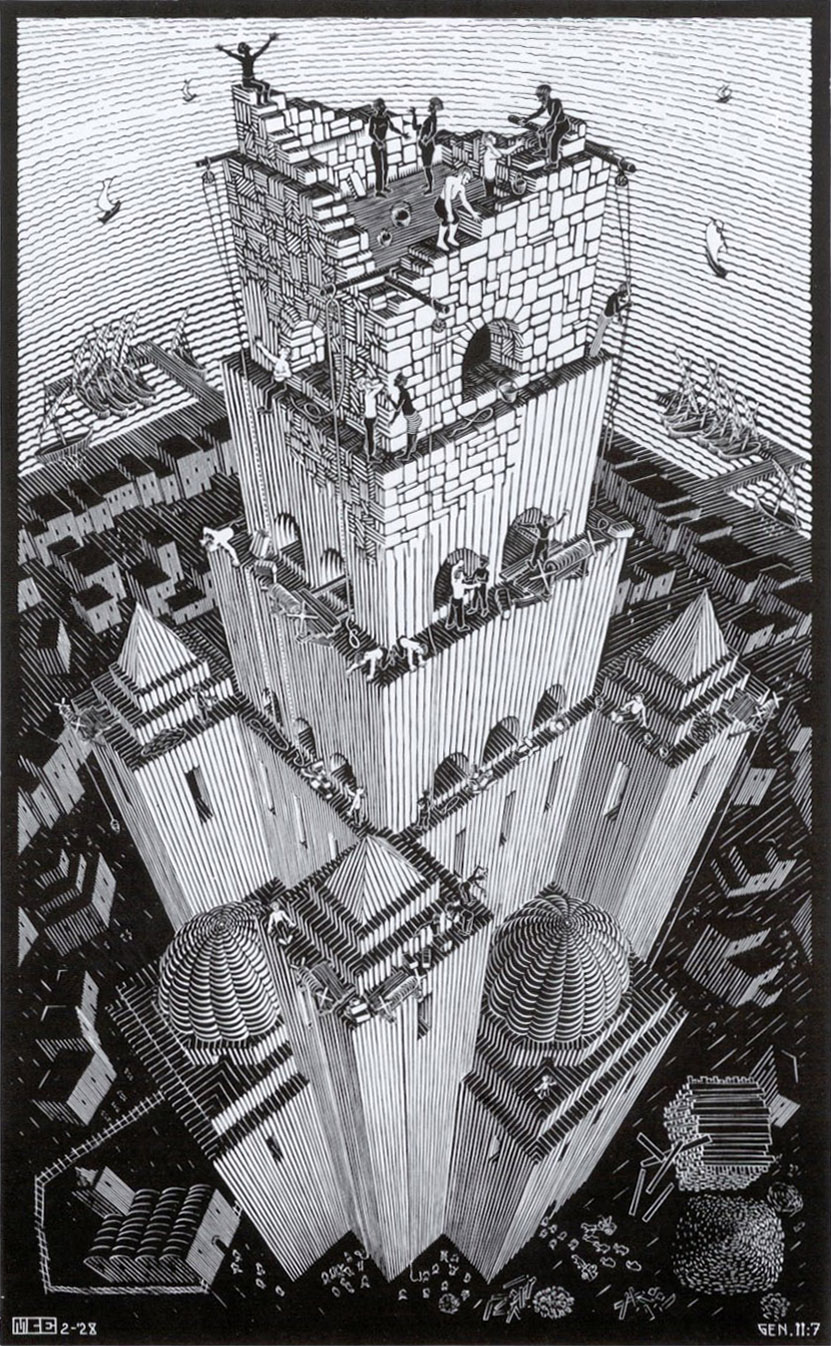
\includegraphics[height=.9\textheight]{img_021.jpg}
\caption[巴别塔,艾舍尔作。]
  {巴别塔,艾舍尔作(木刻,1928)。}
\end{figure}

不过,这种建构的艺术是另外一种类型,不同于——比如说——摩天大楼的建筑(见\fig{21})。对于后者来说,能够矗立在那里,就足以证明它的各个结构要素是紧密组合起来的。但对于一本几何学的书来说,当其中的每个命题都声称是从前面的命题逻辑地推导出来时,若某个命题的证明是无效的,并不会显出整个建构会倒坍。这里横梁和立柱不是物质的,而是抽象的。事实上,在欧几里德的《几何原理》中,用来建构证明的东西是人类语言——一种充满隐患的复杂又难以捉摸的通讯媒介。那么,《几何原理》的建构聚合力是什么呢?能肯定它是由坚固的结构要素组合起来的吗?或者它也许有结构上的弱点?

我们用的每个词对于我们都有某种意义,在我们使用这个词的时候引导我们。越是普通的词,我们由它引起的联想就越多,其意义也就扎得越深。所以,如果某人对一个普通的词下个定义,指望我们遵守这个定义,我们肯定不这么做。相反,我们会在很大程度上无意识地按照另一些东西的引导去做,那些东西是我们的心智在我们与这个词相关联的储备中所发现的。我提及这些是因为这就是欧几里德的《几何原理》中所发生的问题,在那里他试图对诸如“点”、“直线”、“圆”等等普通平常的词下定义。你怎样才能给一个人人都已有了清晰概念的东西下定义?唯一的途径是假定你能清楚地表明你的词是当作术语的,不与同样拼写的日常用词相混淆。你必须得强调:与日常用词的联系仅仅是提示性的。可是,欧几里德没这么做,因为他觉得他的《几何原理》中的点和线的确就是现实世界中的那种点和线。所以,由于没有明确截断所有联系,欧几里德使得读者能自由地发挥他们的联想力了……

这看起来几乎没有秩序可言了,而且对欧几里德也有点不公平。他确实制定了公理,或说公设,可用来证明命题。事实上,除了这些公理公设,别的东西一律不得使用。而就是在这里他失误了:他使用那些日常用词的一个不可避免的后果就是那些词生出的一些意象潜入了他给出的证明。不过,如果你读《几何原理》中的证明,无论如何别指望发现推理中扎眼的“跳跃”。正相反,它们非常精细,因为欧几里德是个思想敏锐的人,在他那里不会出现任何头脑简单所导致的错误。尽管如此,缝隙还是有的,造成了一部经典著作中轻微的瑕疵。但不应抱怨这一点,只应该体会到绝对严格与相对严格之间的差别。毕竟,在欧几里德写下他的著作两千多年以后,他缺乏绝对的严格性这一点导致了数学中一些最富成果的新分支。

欧几里德给出了五条公设作为几何学这个无穷级大厦的“地基”——他的《几何原理》只包括了这个大厦的前几百级。前四条公设相当优美简洁:
\begin{enumerate}
\item 一条直线段可以联接两个点。
\item 一条直线上任何一条直线段可以无限延伸。
\item 给定一条直线段,可以以一个端点为圆心,以此线段为半径做一个圆。
\item 一切直角都彼此相等。
\end{enumerate}
然而第五条却不那么雅致:
\begin{enumerate}[resume]
\item 如果两条直线与第三条直线相交时,在第三条直线的某一侧三条线所夹的内角之和小于两个直角的和,则那两条直线沿着这一侧延伸足够长之后必然相交。
\end{enumerate}

虽然欧几里德从未明白地说过,但他确是把这条公设看得比其它几条地位低些,因为在前二十八个命题的证明里,他想法避免了使用它。这样,前二十八个命题属于所谓“四公设的几何学”——几何学中的一部分,可基于《几何原理》的前四条公设而导出,无需第五条公设的帮助(常常也称作“绝对几何学”)。无疑,欧几里德会发现:更为可取的是证明这只丑小鸭,而不必设定它。但他没找到证明,所以采纳它了。

但是欧几里德的后继者们在不得不设定这第五公设时,并不比他自在些。多少个世纪里,数不清的人花费了他们生命里数不清的岁月,试图去证明第五公设本身便是四公设几何学的一部分。到1763年,至少发表了二十八种不同的证明——都是错的!(都被一个名叫克吕格的人在一篇论文里批驳了)。所有这些错误的证明都涉及到了日常直观与严格的形式化属性的混淆。这么说是保险的:在今天几乎所有这些“证明”对我们都没有什么数学的或历史的价值了——除了几个例外。

\section{非欧几里德几何面面观}

济罗拉莫·萨彻利(1667--1733)生活在巴赫的时代。他有个抱负,要使欧几里德不带任何瑕疵。以他早期在逻辑方面的研究为基础,他决定试着从一个新颖的角度对那个著名的第五公设进行证明:假定你设定它的反面,然后以这样一条公设作为你的第五公设开始推演几何学……肯定不久之后你会制造出矛盾。因为没有任何数学系统能支持矛盾,你就表明了你自己的那个第五公设是不可靠的,于是表明了欧几里德的第五公设是可靠的。这里我们无需深究细节。指出下面这一点就够了:萨彻利以他高超的技巧推演出了“萨氏几何学”的一个又一个命题,最后终于变得厌倦了。有一个时候,他认定他达到了一个“与直线的本质相抵触”的命题。那正是他一直期望的——在他看来,那是个寻找已久的矛盾。就在那个时候他发表了他的研究结果,题为《不带任何瑕疵的欧几里德》,随后就不干了。

但就是因为这么做,他剥夺了自己身后的殊荣,因为他无意中发现了后来所谓的“双曲几何学”。五十年以后,兰伯特重复了这种“失之交臂”,这次,假如能这么说的话,甚至更接近了。最后,兰伯特之后四十年,也即萨彻利之后九十年,非欧几何学被认可了——一个真正的几何学新品种。这是自古以来单一的数学的一个分叉点。1823年,作为那种无从解释的巧合之一,非欧几何同时被两个人发现了。他们是匈牙利数学家雅诺(或约翰)·鲍耶,二十一岁,和俄国数学家尼古拉伊·罗巴切夫斯基,三十岁。具有讽刺意味的是,在同一年法国伟大的数学家阿德里安—马利·勒让德想出了他认定是对欧几里德第五公设的一个证明,他在相当程度上是沿着萨彻利的路子。

顺便指出,鲍耶的父亲法卡斯(或沃夫岗)·鲍耶,伟大的高斯的一个亲密朋友,投入了大量精力试图证明欧几里德的第五公设。在一封给他儿子雅诺的信中,他努力劝阻他不要去思考这种东西:

\begin{quote}
你一定不要去探究平行公设。我深知这条路通向哪里。我曾横穿于这无尽的黑夜,湮灭了我生命中所有的光明与欢乐。我恳求你放下平行公设的研究……我曾想为了真理而牺牲自己。我准备好成为一个殉教者,除去几何学的瑕疵,使之纯净而奉还给人类。我进行了巨大的、难以估量的努力,我得到的结果远比其他人好得多,却依然没达到完全的满意。当一个人彻底离开日常之琐碎,他就转向了崇高之最。当我看出没人能达到这黑夜的尽头时,我转回身了。我转回身来没有慰藉,却带着对自己以及全部人类的怜悯……我旅经了这地狱般的死海里的所有暗礁,总是帆破桅折地回来。就是从那时起,我开始衰老,性情也毁了。我不加考虑地用我的生命和幸福去冒险——或者光荣如凯撒,或者一无所有。\note{赫伯特·梅什科夫斯基[Herbert Meschkowski],《非欧几里德几何学》,第31--32页。}
\end{quote}

但是后来,当他确信他的儿子的确“有了东西”,他便催促他发表,正确地迎来了那个同时性。这种同时性在科学发现上真是屡屡发生:

\begin{quote}
当时机成熟时,那些东西在不同的地方出现,就像早春时的紫罗兰。\note{赫伯特·梅什科夫斯基[Herbert Meschkowski],《非欧几里德几何学》,第33页。}
\end{quote}

非欧几何学的情形真真确确就是这样!在德国,高斯自己和其他一些人都多少独立地触及了非欧几何观念。其中包括一个律师施外卡特,他于1818年寄给高斯一篇文章,描述了一种新的“星际”几何学;施外卡特的侄子陶利努斯做出了非欧几里德三角学;高斯的学生瓦赫特尔,他发现了非欧几何学的几个很深的结果,死于1817年,当时二十五岁。

理解非欧几何的线索是“率直对待”来自像萨彻利和兰伯特的几何学里的命题。只是当你没能摆脱先入为主的“直线”观念时,萨氏命题才“与直线的本质相抵触”。而若你能使自己摆脱那些先入的印象,只让“直线”是那种满足新命题的东西,那你就达到了一个崭新的视点。

\section{未定义项}

这听起来很熟悉。具体地说,让人想起"pq"系统以及它的变种,其中符号借助它们在定理中扮演的角色而获得被动意义。符号"q"尤其令人感兴趣,因为它的“意义”随着新公理的添加而改变了。人们可以以完全相同的方式让“点”、“线”等等的意义由它们出现于其中的定理(或命题)的集合来决定。这是非欧几何学发现者们的重大体会。他们以不同的方式否定欧几里德第五公设,并遵循其后果,从而发现了几种不同的非欧几何学。严格地说,他们(包括萨彻利)并不是直接否定第五公设,而是否定了一个等价的公设。它被称为平行公设,其叙述如下:

\begin{quote}[]
给定任一直线和不在直线上的一点,存在有一条,且仅仅存在一条通过那个点,且永不与前一条直线相交的直线,无论两直线延伸多远。
\end{quote}

第二条直线就称为与前一条直线平行。如果你断言没有这样的直线存在,那么你得到的是椭圆几何学;如果你断言至少有两条这种直线存在,你得到的是双曲几何学。顺便指出,这样的变种还被称为“几何学”的理由是核心要素——绝对的或四公设几何学——嵌于其中。就是由于有这最小限度的核心,把它们当作对某种几何空间性质的描述才有意义,尽管这种几何空间不像平常的空间那么直观。

实际上,椭圆几何学是很容易视觉化的。所有的“点”、“线”之类东西都可认作是普通球面上的东西。让我们来规定一下:作为术语时,我们写“\emph{点}”,作为日常用语时,我们写“点”。现在我们可以说一个\emph{点}由一对球面上的对径点(球的一条直径的两端点)组成。一条\emph{线}是球的一个大圆(一个圆,像赤道那样,以球心为其圆心)。在这种解释下,椭圆几何学的命题虽然也含有“\emph{点}”、“\emph{线}”之类的词,说的却是球面上发生的事情,而不是平面上的。注意:两条\emph{线}总是相交于两个点,两个在球面上对称于球心的点——也就是恰好相交于一个\emph{点}!而且正像两条线决定一个点,两个点也决定一条线。

这种对待“\emph{点}”和“\emph{线}”这些词的方法——即认为它们仅有的意义是那些它们出现于其中的命题灌注进去的——使我们向几何学的完全形式化前进了一步。这种半形式化的版本仍然使用了汉语中的许多词,带有它们通常的意义(像“一个”、“如果”、“和”、“连接”、“有”等词),虽然特殊的词,如“\emph{点}”和“\emph{线}”,其日常意义已被抽掉了。后者于是称作未定义项。未定义项,像"pq"系统中的"p"和"q",在某种意义上是有定义的:它们被隐含地定义了——由它们出现于其中的那些命题全体定义,而不是在一个定义中显明地定义。

人们可以主张说未定义项的完整定义仅驻存于公设中,因为导出的命题已是隐含于公设中了。在这种观点下,公设隐含地定义了所有未定义项,这些定义体现于全部未定义项的相互关系之中。

\section{多重解释的可能性}

几何学的完全形式化需要一个激烈的措施:使每个词项都成为未定的——就是,把每个词项都变成形式系统中“没有意义”的符号。我在“没有意义”上加引号是因为,你也知道,那些符号自动地具有了从它们出现于其中的定理而来的被动意义。不过,人们是否发现了那些意义却是另外一个问题了,因为那将要求寻找这样一集概念,它们能通过同构联系于形式系统中的符号。如果一个人带着把几何学形式化的目的起步,他大概是对每个符号都有了一个意向中的解释,使被动意义铸入系统。这就是我开始构造"pq"系统时对"p"和"q"所做的。

但也许还有其它潜在地可接受的被动意义未被人注意。例如在原来那个"pq"系统中令人意外地把"p"解释成“等于”,把"q"解释成“减”。虽然这个例子很平凡,却包含了这样一个想法的核心:符号可以有许多有意义的解释——寻找它们是取决于观察者的。

我们可以用术语“一致性”来概括到目前为止我们的考察。我们的讨论开始于虚构一个显得不一致的形式系统——内部不一致,同样与外部世界也不一致。但过了一会我们就撤回了这种说法,我们意识到了我们的错误:我们为符号选择了不幸的解释。改换了解释以后,我们重新获得了一致性!现在很清楚了:一致性不单是形式系统的性质,还依赖于为之提出的解释。同理,不一致性也不是任何形式系统的固有性质。

\section{各种各样的一致性}

我们一直在谈论“一致性”和“不一致性”,却还没定义它们。我们只是依靠古老悠久的日常观念。现在让我们来严格地定义一个形式系统(加上一个解释)的一致性:这是指其中每个定理经解释后都成为一个真陈述。如果至少有一个经解释后的定理是假陈述,我们就说出现了不一致性。

这个定义似乎是在谈论系统与外部世界的不一致性。那么,内部的不一致性怎么样呢?大概是如果一个系统含有两个或更多的定理,其解释是彼此不相容的,那么它是内部不一致的;而若所有经解释后的定理彼此相容,则是内部一致的。作为一个例子,让我们考虑一个形式系统。它只有下述三个定理:"WdZ"、"ZdG"、"GdW"。如果"W"解释成“乌龟”,"Z"解释成“芝诺”,"G"解释成“吉世达”,而$x"d"y$解释成“$x$总是在下棋时打败$y$”,那么我们就有了下列经解释后的定理:
\begin{itemize}
\item 乌龟总是在下棋时打败芝诺。
\item 芝诺总是在下棋时打败吉世达。
\item 吉世达总是在下棋时打败乌龟。
\end{itemize}
陈述本身并非不相容,虽然它们描述了一个相当怪诞的棋手圈子。所以,在这个解释下,以那三个符号串为定理的形式系统是内部一致的,虽然实际看来那三个陈述没一个是真的!内部一致性不要求所有的定理都得成为真陈述,只需它们能成为彼此相容的陈述。

现在假定我们把$x"d"y$另外解释成“$x$是$y$笔下的人物”,那么我们就有:
\begin{itemize}
\item 乌龟是芝诺笔下的人物。
\item 芝诺是吉世达笔下的人物。
\item 吉世达是乌龟笔下的人物。
\end{itemize}
在这种情况下,单个的陈述是真是假没有关系——恐怕也没有什么办法能知道哪些是真哪些是假。不过,肯定不会是它们三个同时都真。这样,这个解释就使系统内部地不一致了。这个内部的不一致性不取决于对那三个大写字母的解释,而仅仅取决于对"d"的解释,同时还取决于那三个大写字母是循环地排列于"d"的各次出现周围这一事实。于是,人们可以不必解释形式系统的所有符号而找到内部不一致性(在这个例子里,单解释一个符号就够了)。到了足够多的符号都有了解释的时候,可能就会清楚地看出:没有什么解释其余符号的办法能使所有的定理成为真的。但这不仅是真假的问题——这是个可能性的问题。如果我们把大写字母都解释成真人的名字,三个定理就都成了假的——但那不是把系统称作内部不一致的理由。我们的根据是循环性,再加上对字母"d"的解释。(顺便提醒一句,你会在第二十章再见到这个“作者三角形”)。

\section{假想的世界和一致性}

我们给出了两种看待一致性的方式:前一个说,如果每个定理经解释后成为真的,则系统加上解释是与外部世界一致的;后一个说,如果所有的定理经解释后成为彼此相容的,则系统加上解释是内部一致的。这两种类型的一致性之间有密切的关系。为了决定几个陈述是否彼此相容,你得设法想象一个世界,在其中它们能同时都真。所以,内部的一致性有赖于与外部世界的一致性——只是现在,“外部世界”允许是任何想象的世界,而不必是我们生活于其中的那个世界。但这是一个极其模糊的、无法令人满意的结论。一个“想象”的世界都有些什么东西?是否可能想象一个世界,在其中三个人物是循环地相互创造出来的?是否可能想象一个世界,其中有方的圆?这样一个世界是不是可想象的:其中是牛顿定律而非相对论成立?是否可能想象一个世界,其中有绿的并且又不是绿的东西?或者这样一些世界:其中的动物不是细胞组成的、在其中巴赫在腓特烈大帝的主题上即兴演奏了八声部赋格曲、在其中蚊子比人更聪明、在其中乌龟能踢足球——或谈论足球?当然了,一只谈论足球的乌龟的确有点反常。

这些世界里,有一些似乎比另一些更可想象,因为有些世界似乎包含了逻辑矛盾——例如,绿的并且又不是绿的。而另一些似乎是——找不到更好的词——“说得通的”,例如巴赫即兴演奏八声部赋格曲、存在不是由细胞构成的动物。甚至可以设想一个有不同物理定律的世界……因此,大体上该是有可能建立不同品种的一致性。举个例子来说,最宽松的会是“逻辑一致性”:对事物不加任何制约,只对逻辑有所要求。更具体地说就是一个系统加上解释是“逻辑一致”的,仅当它其中没有任何两个定理在解释成陈述时直接地相互矛盾;“数学一致”的,仅当经解释后的定理不违背数学;“物理学一致”的,仅当所有经解释后的定理与物理法则相容;“生物学一致”的……如此等等。在一个生物学一致的系统里,可以有这样的定理,其解释是陈述“莎士比亚写了一部歌剧”,但不会有定理其解释是陈述“存在无细胞动物”。一般说来,这类玄想出来的不一致性没什么人去研究,原因是很难把它们一个个理清楚。举例来说,三个人物循环地互相创造这个问题涉及的不一致性应该说是哪一种?逻辑的?物理学的?生物学的?文学的?

通常,有意思和没有意思之间的分界线是画在数学一致性和物理学一致性之间的。(这当然是数学家和逻辑学家们画的了——很难说他们是一个不带偏见的群体……)这意味着对于形式系统来说,只有数学和逻辑类型的不一致性才“算数”。若按照这个约定,那么我们就还没有找出一个解释,使那个三定理组"WdZ"、"ZdG"、"GdW"不一致。这一点可以通过把"d"解释成“大于”来做到。"W"、"Z"和"G"怎么办?它们可以解释成自然数——比如,"Z"是$2$,"W"是$3$,"G"是$6$。注意这种解释下有两个定理成为真的,有一个假的。如果我们另外把"Z"解释成了$8$,就会有两个假的,仅有一个真的了。但两者都使我们得到了不一致性。事实上,指派给"W"、"Z"和"G"的值是无关紧要的,只要明白需限制在自然数范围内。我们又一次看到这种情形:为了认出内部不一致性,只需要某些解释。

\section{形式系统中嵌入形式系统}

前面那个例子,其中某些符号可以在其余符号没有解释的情况下具有解释,让人想起在自然语言里构造几何学时,使用的某些词是未定义项。在这种情况下,词就可以分成两类:一类词有固定不变的意义,另一类词的意义有待调整,直到系统成为一致的(这一类是未定义项)。用这种方式构造几何学,要求第一类词的意义已经在几何学之外制定好。这些词构成一个刚性的骨架,赋予系统一个基础结构;填充那个骨架的是其它材料,它们是可以改变的(欧氏或非欧几何学)。

形式系统常常就是以这种相继的、或者说分层的方式构造出来的。举例来说,形式系统I设计好了,有一些规则和公理,它们赋予符号以某种意向的被动意义。然后形式系统I完全合并到一个有更多符号的更大的系统里——形式系统II。由于形式系统I的公理和规则是形式系统II的一部分,形式系统I的符号的被动意义仍然有效。它们构成一个不变的骨架,随后便在决定形式系统I的新符号的被动意义时起很大的作用。然后,或许会轮到第二个系统对第三个什么系统起骨架的作用,如此下去。也可能——几何学就是个很好的例子——有一个系统(例如绝对几何学),它部分地固定住其中的未定义项的被动意义,并能对其添加另外的规则或公理,以进一步地限定那些未定义项的被动意义。这就是欧氏与非欧几何学的情形。

\section{视知觉中的稳定性层次}

我们获得新知识、新词汇,或感知不熟悉的事物,都是以与此类似的分层方式进行的。尤其有趣的是理解艾舍尔的画时的情形。比如,《相对性》(\fig{22})中出现了简直是不可能的景象。你也许认为我们会一遍又一遍地力求重新解释这幅画,直到我们把它的各个部分解释成没有矛盾的——但我们根本不那么做。我们坐在那里,看着那些通向各处的楼梯和那些在同一楼梯上沿着不一致的方向走动的人们,又愉快又困惑。那些楼梯是些“确定性的岛屿”,我们对整幅画的解释就以它们为基础。一旦确定了它们,我们就试图扩展我们的理解,去探求它们彼此之间的关系。就是在这一步骤我们遇上了麻烦。但如果我们想要回溯——就是说,对“确定性的岛屿”质疑——我们也会遇上麻烦,只不过是另一种麻烦而已。没有什么通过回溯否认它们是楼梯的办法。它们不是鱼、鞭子或手——它们就是楼梯(实际上有另外一个办法——让画中的所有线条都完全没有解释,就像形式系统中的“没有意义的符号”。这种彻底的逃避途径是“"U"方式”反应的一个例子——一种对待符号表示的禅宗式态度)。

\begin{figure}
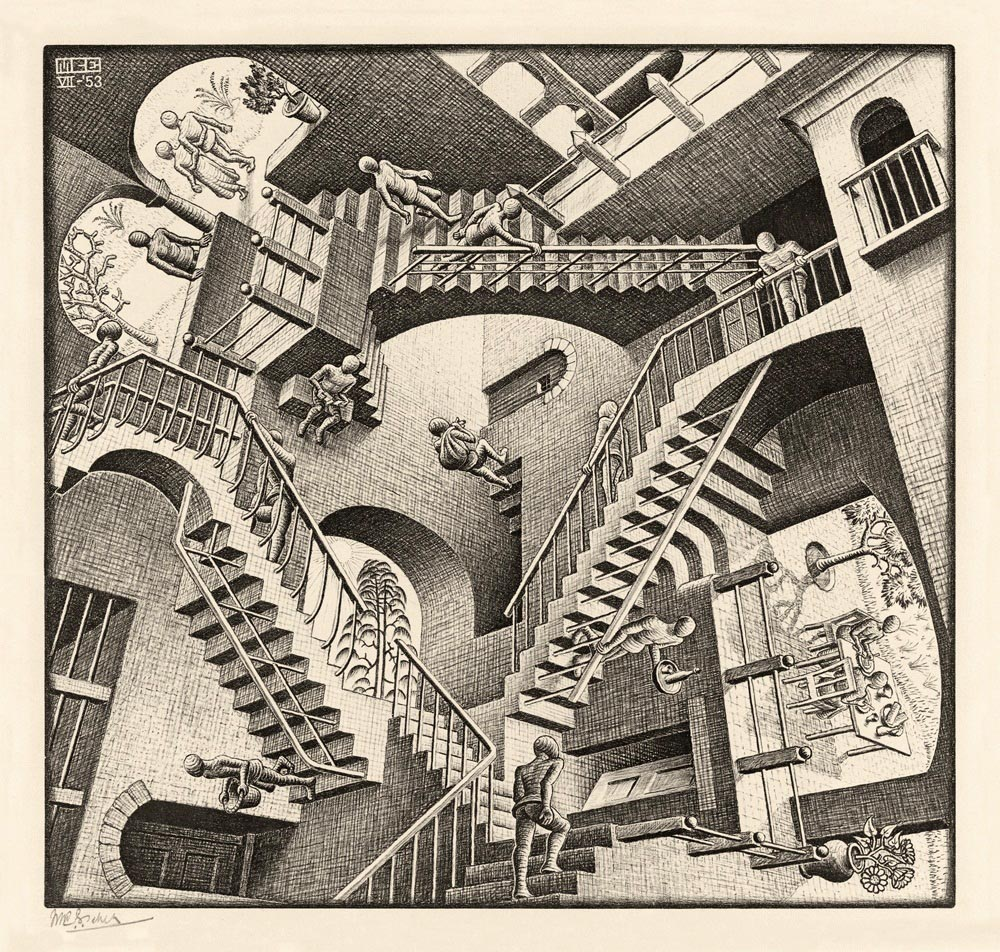
\includegraphics{img_022.jpg}
\caption[相对性,艾舍尔作。]
  {相对性。艾舍尔作(版画,1953)。}
\end{figure}

由于我们知觉过程的层级性质,我们被迫或者看到一个疯狂的世界,或者看到一簇毫无意思的线条。相似的分析可用于艾舍尔的许多画,它们都大量地依赖于对某些基本形状的识别,然后再以非标准的方式组合在一起。到观众在高层上看出悖谬的时候,就已经太晚了——他无法再回去,对怎样解释较低层次的对象改换想法。艾舍尔的画与非欧几何学的区别在于:对于后者,能找到对未定义项的可理解的解释,得出一个可理解的完整系统;而对于前者,无论盯着画看多长时间,最后的结果与人们关于世界的概念仍不可调和。当然,人们仍然可以虚构假想的世界,在其中艾舍尔的那类事件能够发生……但是在那样的世界里,生物学、物理学、数学甚至逻辑的法则会在一个层次上被违反而同时在另一个层次上被遵循,使之成为一个极其古怪的世界(例子之一是《瀑布》(\fig{5}),那里面正常的引力适用于流动的水,但空间的性质却违反了物理学原理)。

\section{数学在每个可想象的世界里都是一样的吗?}

上面我们强调过,形式系统(加上一个解释)的内部一致性要求存在某种想象的世界——对这类世界唯一的限制是其中的数学和逻辑与我们的世界一样——在其中所有经解释后的定理都成为真的;而外部的一致性——与外部世界的一致性——则要求所有的定理在现实世界里都成为真的。现在来看一个具体情形。一个人希望构造一个一致的形式系统,其定理要解释成数学陈述,那么看起来两种类型的一致性之间的区别就消失了,因为,如上所说,所有想象的世界都有与现实世界一样的数学。于是,在每个可想象的世界里,$1$加$1$必须是$2$;同样,必须存在无穷多的素数;进一步,在每个可想象的世界里所有直角都必须是相等的;而且当然还有:经过任一不在给定直线上的点,必是恰有一条与之平行的直线……

但等一下!那可就是平行公设——断言其普遍性将是个错误,这我们刚刚说过。如果所有可想象的世界都遵循平行公设,那就是断言非欧几何是不可想象的,我们就又回到了萨彻利和兰伯特的心理水平了——肯定是不智之举。但什么车西,如果不是所有数学,必须是所有可想象的世界共有的?会是少到逻辑本身吗?或甚至逻辑也是可疑的:是否有那种世界:矛盾是存在的正常组成部分——矛盾在那里不是矛盾?

从某种意义上讲,仅仅作为发明出来的概念,我们已表明这种世界是可想象的;但在更深一层的意义上讲,它们是很不可想象的(这本身又是个小矛盾)。然而,认真地讲,如果我们想要有所交流,看来就得采纳某种共同基础,而逻辑几乎总是得包括进来的。(有些信仰系统是拒斥这种观点的——它太逻辑化了。具体说来,禅宗就是以同等的热情拥抱矛盾和非矛盾的。这似乎不太一致,但不一致也是禅宗的一部分,所以……你能说什么呢?)

\section{数论在每个可想象的世界里都是一样的吗?}

如果我们假定逻辑是每个可想象世界的一部分(注意,我们还没有给逻辑下定义,但我们会在以后的章节里给出来),是否就行了?真的能想象某些世界没有无穷多素数吗?所有可想象的世界里,数应该遵循同样的法则,这难道不是必要的吗?或者……把“自然数”这个概念也当作未定义项,就像“\emph{点}”或“\emph{线}”,是不是更好些?那样的话,数论就是个分叉的理论了,像几何学一样:就会有标准数论和非标准数论了。但要有与绝对几何学相应的某种东西:一个“核心”理论,一个所有数论的不变组成部分,以确认数论是数论,而不是关于——比如说,可可或橡皮或香蕉的理论。存在这样的一个核心数论,它应该与逻辑一起包含在我们认为是“可想象的世界”里,这似乎是大多数当代数学家和哲学家的共识。这个数论的核心——绝对几何学的对应物——被称作皮亚诺算术,我们会在第八章里形式化地给出来。另外,现在已经很明朗——实际上是哥德尔定理的直接后效——数论是分叉的理论,有标准的和非标准的版本。然而,与几何学的情形不同,数论的“品种”有无限多个。这使得数论的情形变得极其复杂。

从实际应用的角度看,所有的数论都是一样的。换句话说,如果桥梁的建造依赖于数论(在某种意义上确实如此),那么,不同的数论的存在不会造成什么影响,因为在与现实世界有关的那些方面,所有的数论都是重合的。对不同的几何学可不能这么说。例如,三角形的内角和只在欧几里德几何中是$180$度,在椭圆几何中要大于这个值,而在双曲几何中要小于这个值。据说高斯曾试图测量三座山峰所形成的三角形的内角和,以最终确定我们的宇宙到底服从哪种几何学。直到一百年后,爱因斯坦提出了一种理论(广义相对论),认为宇宙的几何性质是被其内含的质量所确定的,因此没有哪种几何是空间自身所固有的。所以,对“哪种几何学是正确的?”这个问题,自然界不仅在数学中,而且也在物理学中给出了一个模棱两可的答案。至于那个与此对应的问题“哪种数论是正确的?”,当我们详细地介绍了\emph{哥德尔定理}后,还会有更多的话要说。

\section{完全性}

如果一致性是符号获得被动意义的最低条件,那么与之互补的概念,完全性,是那些被动意义的最高确认。一致性是说:“系统产生的每个东西都是真的”,完全性是倒过来:“每个真陈述都是由系统产生的”。现在稍稍修饰一下这个概念。我们不会是指世界上所有的真陈述——我们指的仅是这样的陈述:它们所属的领域是我们力图用该形式系统去表达的。所以,完全性的意思是:“每个能由系统中的概念表示出来的真陈述都是系统中的定理”。
\begin{thm}{一致性}
每个定理经解释后都成为真的(在某个想象的世界里)。
\end{thm}
\begin{thm}{完全性}
所有真的(在某个想象的世界里)且可表示成系统中的良构符号串的陈述都是定理。
\end{thm}
最初那个"pq"系统以及它原来那个解释是这种形式系统的一个例子:它在自己那谦逊的水平上是完全的。任何两个正整数的正确的加法式子都可表示为系统中的定理。我们也可以换一种方式来说:“任何两个正整数的加法式子都是在系统内可证的”。(小心:当我们开始用“可证的陈述”而非“定理”这种说法时,表明我们开始混淆形式系统与其解释之间的区别。这是可以的,只要我们清楚地意识到这种混淆出现了,并且记得多重解释有时是可能的。)"pq"系统加上它原来那个解释是完全的;同样也是一致的,因为没有假陈述——用我们的新说法——是在系统内可证的。

有人可能会争辩说这个系统是不完全的,根据是三个正整数的加法式子(如$2+3+4=9$)没有被"pq"系统的定理所体现,尽管能翻译成系统中的概念(例如,$---------"q"--"p"---"p"----$)。然而,这个符号串不是良构的,因此我们认为它就像$"pqp"---"qpq"$一样缺乏意义。三个数的加式用系统中的概念根本不可表示——所以系统还是有完全性的。

尽管"pq"系统在这种解释下有完全性,离完全地捕捉数论中的真理当然还差得远。比如,"pq"系统就没有办法告诉我们有多少素数存在。\emph{哥德尔不完全性定理}说的是任何“足够强有力”的系统,由于其能力较强,因而是不完全的。即:存在良构的符号串,表示了数论中的真陈述,但不是定理(有属于数论的真陈述在系统内不可证)。"pq"系统这样的系统是完全的,但能力不强。它们更像是低保真的唱机:太贫乏了,很明显做不了我们想要它们做的——即告诉我们数论中的每件事实。

\section{一个解释怎样就能达到或破坏完全性?}

那么所谓“完全性是被动意义的最高确认”——我在前面这么说过——是什么意思呢?意思是:如果一个系统是一致的,但不完全,符号和其解释之间就会错配。系统没有能力为那样的解释作辩护。有时,如果把解释稍稍“修剪”一下,系统就会变得完全。为说明这个思想,让我们来看看修改的"pq"系统(含有公理模式II)及我们对它的解释。

修改了"pq"系统之后,我们把"q"的解释从“等于”修改为“小于或等于”。我们看到,修改的"pq"系统在这种解释下是一致的,但新解释却有些令人不太满意的地方。问题很简单:现在有许多可表示的真陈述不是定理。例如,“$1$小于或等于$2$加$3$”表示成非定理$-"q"--"p"---$。这个解释实在是太不彻底了!它没有精确地反映出定理在系统中的作为。我们可以这样来纠正:或者\pnum{1}向系统添加新规则,使之增强能力,或者\pnum{2}紧缩解释。在这里,明智的选择看来是紧缩解释。不把"q"解释成“小于或等于”,而代之以“等于或加$1$后等于”。现在,修改后的"pq"系统变得既是一致的又是完全的,而完全性确保了这个解释是恰当的。

\section{形式化数论的不完全性}

在数论里我们会再次碰到不完全性。但在那里,为了挽救局面,我们被推向另一方向——增加新规则,使之增强能力。具有讽刺意味的是,每次我们增加一条新规则,我们就想,现在我们肯定使系统完全了!这种困境的性质可由下述类比来说明……

我们有一台唱机,还有一张唱片,上面标着“基于B-A-C-H的卡农”。然而,当我们把唱片放在唱机上播放时,由反馈引起的震颤(与乌龟的唱片引起的震颤一样)干扰得太厉害,以致于我们甚至都辨不清曲调了。我们断定某个东西有缺陷——不是唱片就是唱机。为了检测我们的唱片,我们就得到朋友的唱机上去播放,听它的质量。为了检测我们的唱机,我们就得用朋友的唱片在其上播放,看看我们听到的音乐是否符合标签。如果我们的唱机通过了对它的检测,则我们就说是唱片有缺陷;反过来一样,如果唱片通过了对它的测试,则我们就说是唱机有缺陷。然而,若结果是两者分别通过了对它们的测试,我们作什么结论呢?现在正是时候:回忆一下那两个相继的同构(\fig{20}),仔细想想!
